%%
%% This file is `Final_Paper_NL.tex',
%% modeled on the example sample-xelatex.tex provided
%% by the ACM.
%% The first command in your LaTeX source must be the \documentclass command.
\documentclass[sigconf]{acmart}
\usepackage{booktabs}
%%
%% \BibTeX command to typeset BibTeX logo in the docs
%\AtBeginDocument{%
%  \providecommand\BibTeX{{%
%    \normalfont B\kern-0.5em{\scshape i\kern-0.25em b}\kern-0.8em\TeX}}}

%% Rights management information.  This information is sent to you
%% when you complete the rights form.  These commands have SAMPLE
%% values in them; it is your responsibility as an author to replace
%% the commands and values with those provided to you when you
%% complete the rights form.
\setcopyright{acmcopyright}
\copyrightyear{2021}
\acmYear{2021}
\acmDOI{TBD}

%% These commands are for a PROCEEDINGS abstract or paper.
\acmConference[Conference TBD]{Conference TBD}{Location, TBD}
\acmBooktitle{Book info TBD}
\acmPrice{Price TBD}
\acmISBN{ISBN TBD}


%%
%% Submission ID.
%% Use this when submitting an article to a sponsored event. You'll
%% receive a unique submission ID from the organizers
%% of the event, and this ID should be used as the parameter to this command.
%%\acmSubmissionID{123-A56-BU3}

%%
%% The majority of ACM publications use numbered citations and
%% references.  The command \citestyle{authoryear} switches to the
%% "author year" style.
%%
%% If you are preparing content for an event
%% sponsored by ACM SIGGRAPH, you must use the "author year" style of
%% citations and references.
%% Uncommenting
%% the next command will enable that style.
%%\citestyle{acmauthoryear}

%%
%% end of the preamble, start of the body of the document source.
\begin{document}

%%
%% The "title" command has an optional parameter,
%% allowing the author to define a "short title" to be used in page headers.
\title{Vocabulary Entropy in Reddit discussions of US Politics}

%%
%% The "author" command and its associated commands are used to define
%% the authors and their affiliations.
%% Of note is the shared affiliation of the first two authors, and the
%% "authornote" and "authornotemark" commands
%% used to denote shared contribution to the research.
\author{Nicholas A. Lines}
\authornote{This work was completed as a project for a course taught by Ian A. McCulloh.}
\email{nicholasalines@gmail.com}
\orcid{ORCID TBD}
\author{Ian A. McCulloh}
\authornotemark[1]
\email{imccull4@jhu.edu}
\affiliation{%
  \institution{Johns Hopkins University}
  \streetaddress{3400 North Charles Street}
  \city{Baltimore}
  \state{Maryland}
  \country{USA}
  \postcode{21218}
}

%%
%% By default, the full list of authors will be used in the page
%% headers. Often, this list is too long, and will overlap
%% other information printed in the page headers. This command allows
%% the author to define a more concise list
%% of authors' names for this purpose.
\renewcommand{\shortauthors}{Lines and McCulloh}

%%
%% The abstract is a short summary of the work to be presented in the
%% article.
\begin{abstract}
  Distance reading and text mining applications have suggested the need for more language-agnostic techniques
  that can be employed in text analysis. We propose the application of vocabulary entropy to characterize groups of authors,
  and use this approach to analyze and contrast US political discussions carried out on the social media platform
  Reddit. We show that normalized sample mean vocabulary entropy of a community corresponds well with education and literacy
  level, and that vocabulary entropy in political forums varies widely by forum.
\end{abstract}

%%
%% The code below is generated by the tool at http://dl.acm.org/ccs.cfm.
%%
\begin{CCSXML}
<ccs2012>
   <concept>
       <concept_id>10003033.10003106.10003114.10003118</concept_id>
       <concept_desc>Networks~Social media networks</concept_desc>
       <concept_significance>500</concept_significance>
       </concept>
   <concept>
       <concept_id>10002951.10003227.10003351</concept_id>
       <concept_desc>Information systems~Data mining</concept_desc>
       <concept_significance>500</concept_significance>
       </concept>
   <concept>
       <concept_id>10010147.10010178.10010179</concept_id>
       <concept_desc>Computing methodologies~Natural language processing</concept_desc>
       <concept_significance>300</concept_significance>
       </concept>
 </ccs2012>
\end{CCSXML}

\ccsdesc[500]{Networks~Social media networks}
\ccsdesc[500]{Information systems~Data mining}
\ccsdesc[300]{Computing methodologies~Natural language processing}


%%
%% Keywords. The author(s) should pick words that accurately describe
%% the work being presented. Separate the keywords with commas.
\keywords{social media analysis, text mining}

%% A "teaser" image appears between the author and affiliation
%% information and the body of the document, and typically spans the
%% page.
\begin{teaserfigure}
  \centering
  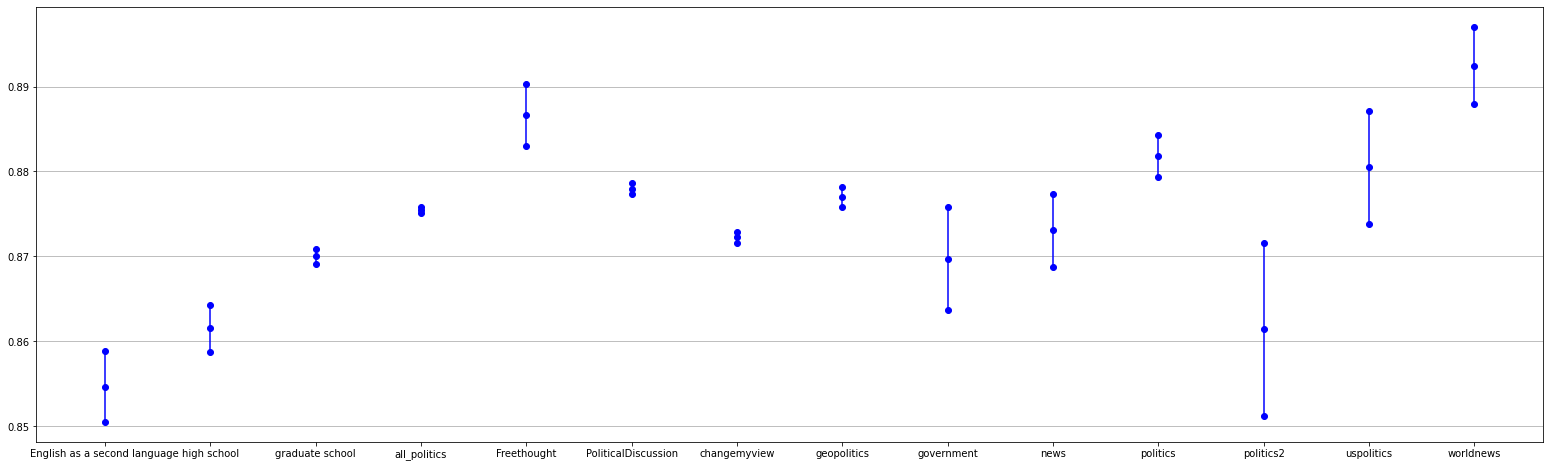
\includegraphics[width=\textwidth]{images/confidenceintervals}
  \caption{Confidence intervals for the mean vocabulary quotient.}
  \label{fig:teaser}
  \Description{We show here the 95\% confidence intervals for the
    mean population vocabulary quotient of various subreddit groups.}
\end{teaserfigure}

%%
%% This command processes the author and affiliation and title
%% information and builds the first part of the formatted document.
\maketitle

\section{Introduction}

As the amount of text-based media has ballooned in recent decades, it has
become clear that the ability to characterize and discuss text corpora at an
abstract level is essential. In the literary community this arose as the
concept of distance reading, in which literary analysis is pursued without
using human judges to actually read books \cite{moretti2000conjectures}. In the
statistics and data science communities we find this problem addressed by
various text mining and authorship verification techniques. The popularity
of topic modeling and other language-agnostic techniques suggests that there
is a rising market for universal methods for characterizing author groups
and text corpora without relying on language-specific features. 

A potentially rich area for research is vocabulary analysis, since all
written language relies on a lexicon of vocabulary. Vocabulary size,
independent of the exact selection of words in that vocabulary, has long
been strongly correlated with mental maturity and other features of interest
such as fluency in one or more languages, education level, etc. \cite%
{nation1993vocabulary}\cite{fox1949some} \ Efforts to measure the true size
of individuals vocabularies, however, tend to be onerous: a recent online
study with almost 300,000 participants tested vocabulary sizes of Dutch
speakers, checking their knowledge of words against a dictionary 53,000
words in length \cite{keuleers2015word}. An alternative to vocabulary size
estimation is the much simpler task of vocabulary entropy measurement, since
the variety in word use is dependent on the number of words known. We
propose that groups of authors can be effectively described in terms of
vocabulary entropy. Using a dataset of English Reddit posts and comments, we
show that vocabulary entropy is related to education and fluency levels, and
then use this tool to explore the landscape of US politics discussion forums
on Reddit. 

\section{Background}

\subsection{Related work}

To the best of our knowledge, this is the first discussion published on the
subject of author group characterization using vocabulary entropy. However,
vocabulary has long been a subject of interest in similar studies.
Authorship verification in academic and court evidence has often relied on
vocabulary analysis, including measures of vocabulary richness \cite%
{chaski2001empiricaleo}. Some of Claude Shannon's original work in entropy
was motivated by a study of variety in English character use \cite%
{shannon1951prediction}. In 2000 the authors of \cite{dale2000handbook}
discussed several measures of vocabulary richness in the context of author
identification, including normalized Shannon entropy. In 2018 an identical
approach for measuring a single author's vocabulary richness was
independently proposed in \cite{rajput2018novel}, and called the \emph{%
vocabulary quotient}. It is important to note that both publications
described this normalized entropy measure as independent of the length of
the text in words, and this is not the case: the vocabulary quotient still
decreases with sample size. However, we will use the vocabulary quotient
throughout this work to remain consistent with the most recent publications
related to the subject.

\subsection{ Vocabulary quotients}

Let $n$ be the length in words of a text sample composed using $V$
distinct words $X_{1},X_{2},...,X_{V}$. These words's frequencies are
observed and used to write the vocabulary's empirical probability
distribution for the random variable for word choice, $X$. The Shannon
entropy of the document is defined to be%
\[
H(X)=-\sum_{i=1}^{V}P(X_{i})\log _{10}P(X_{i}).
\]%
However, vocabulary use in writing follows Heap's law, which states that the
number of unique words observed, $V,$ in a document of length $n$ words is
given by%
\[
V(n)=\alpha n^{\beta },
\]%
where $\alpha $ and $\beta $ are parameters dependent on the author(s) and
possibly the language and context of the document. This means that document
length will greatly affect the entropy measure. As in \cite{dale2000handbook}%
, \cite{rajput2018novel} we use the vocabulary quotient $\frac{H(X)}{-\log
_{10}\left( 1/n\right) },$ the entropy divided by the maximum entropy of a
document of the same size, to dampen this effect, and also restrict our
review to universal fixed sizes of $n$ to ensure true consistency in entropy
measures.

\section{Methodology}

\subsection{Data collection}

Reddit is a social media microblogging platform that consists of many
individual communities called subreddits, whose posts are focused on a
particular subject. Users may post original content, links, etc, and also
provide comments on posts. Using the Python Reddit API\ Wrapper
(\href{https://praw.readthedocs.io/en/latest/}{PRAW}),
we collected samples of the most recent posts and comments from groups of
subreddits associated with non-native English speakers, high school
students, graduate school students, and US\ politics. Since some of the
subreddits surveyed are sparsely used, some of the collected posts date as
far back as 2012, though most occur in spring of 2021. Each post or comment
was tokenized using the NLTK "casual tokenize" strategy (designed for
processing English Twitter data), after having its punctuation and any
handles (user names) stripped and the casing leveled. Any post shorter than
150 tokens was discarded, and the remaining posts were truncated to the
first 150 tokens. The resulting sample sizes are shown in Table ~\ref{tab:sizes}.


\begin{table}
  \caption{Subreddit sample sizes}
  \label{tab:sizes}
  \begin{tabular}{ll}
  \toprule
  Subreddit group & Sample size \\
  \midrule
  English as a second language & 261 \\ 
  High school & 496 \\ 
  Graduate School & 2370 \\ 
  All political subreddits below & 11937 \\ 
  Freethought & 98 \\ 
  PoliticalDiscussion & 4576 \\ 
  changemyview & 5345 \\ 
  geopolitics & 1246 \\ 
  government & 62 \\ 
  news & 81 \\ 
  politics & 314 \\ 
  politics2 & 54 \\ 
  uspolitics & 66 \\ 
  worldnews & 95\\
  \bottomrule
  \end{tabular}
\end{table}

\subsection{Vocabulary quotient computation}

The vocabulary quotient was then computed for each sample text, and the
means recorded for each subreddit group. We found a 95\% confidence interval
for each subreddit group's true mean vocabulary quotient using the sample
variances and the Normality of the sample means. The resulting distributions
are shown in Figure ~\ref{fig:distributions}. We also processed the comments and posts
individually, and found that the mean vocabulary quotient of comments was
usually higher than that of the original posts. We repeated the experiment
with sample sizes of $n=100$ but did not observe any significant difference
in the results.
\begin{figure*}
  \centering
  \setlength\fboxsep{0pt}
  \setlength\fboxrule{0.25pt}
  \fbox{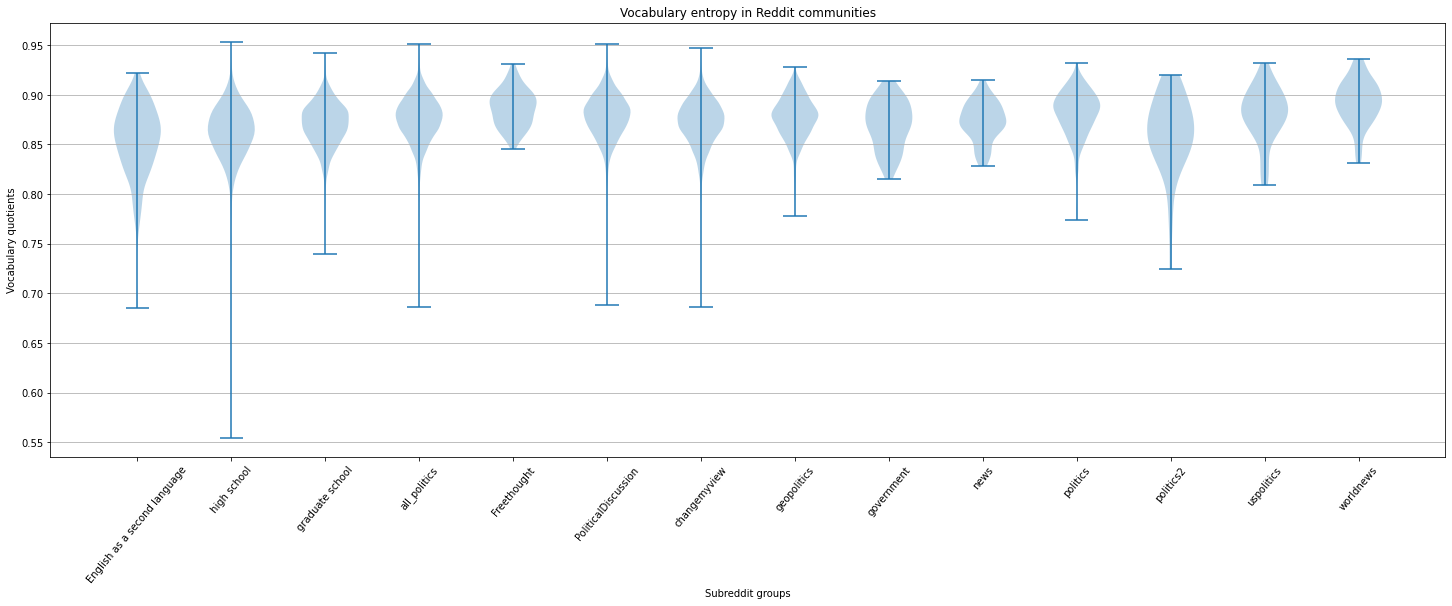
\includegraphics[width=\textwidth]{images/subredditdistributions}}
  \caption{Distributions of vocabulary quotients in various subreddit groups.}
  \label{fig:distributions}
  \Description{These violin plots show the distribution of vocabulary quotients in
    each of the subreddit groups examined in this study.}
\end{figure*}

\section{Results}

\subsection{Analysis}

The confidence intervals for population means of the subreddit groups, given
our samples, are shown in Figure ~\ref{fig:teaser}. This confirms our expectation that
the casual conversation of graduate students exhibits higher vocabulary
entropy than that of high school students or English learners in similar
forums (note that we do not introduce any professional or formal writing, such as essays or
dissertations, but instead restrict our review to Reddit-style conversations). The
distribution of high-school speech is extremely broad, suggesting that
students with high vocabulary entropy show that potential before college
education. 

To our surprise the political discussion subreddits, on average, show higher
vocabulary entropy than any of the above student groups, suggesting more
linguistic sophistication in the discussion content. Individual subreddits
vary, of course, with some closer to high-school level writing and others
significantly higher than graduate school level writing. There are several
environmental facts that may contribute to the unusually high scores.
The highest performing
subreddit, worldnews, is mainly devoted to linking and quoting news
articles rather than posting original content, so it is not surprising that
its vocabulary entropy is similar to that of professional writing. In
contrast, politics2 is a subreddit frequented by users posting from a
variety of world regions and contains much more original, informall
content, which may explain its extremely low vocabulary entropy. 

\subsection{Future Work}

These first steps into vocabulary analysis of social media groups suggest
many further areas to investigate. While we did not explicitly check for
duplication in the data collection process, we did review the results to
show that there were not any frequently occurring quotient values, so it
appears this is a minor concern. However, many subreddits have official and
unofficial bots that create posts and comments, and these may well be
artificially boosting the group's mean quotient. We might also control for
quotations and group-authored content, since this is known to exhibit higher
vocabulary entropy. Improvements could also be made in the text cleaning
approach such as requiring a dictionary lookup, since we found some hyperlinks and
emojis slipped through the casual tokenizer. Despite this fault, the
highest scoring posts and comments in our data were found to genuinely
exhibit diverse vocabulary and more professional writing. 

A severe limitation of all micro-blogging data is the minimal length of
posts hosted by the platforms. Because the length filtering could not occur
within PRAW's scraping routines, over 87\% of the collected posts and
comments collected had to be discarded. This sampling bias toward unusually
long posts means that our analysis is not actually representative of the
whole Reddit community. There could easily be entirely different behavior among
the authors of shorter comments and posts. Another important question to
investigate is just how low
the sample size $n$ can be dropped before the vocabulary quotient is
uninformative. 

Since Reddit is principally a home for informal writing, it would be
informative to contrast these results with samples from more formal writing
such as student essays, LinkedIn posts, or school blogs. How much an
individual or group vary their vocabulary entropy when switching from
informal to formal settings is a question of interest. And finally, we also
wish to investigate the variance of vocabulary quotients across multiple
languages.

\section{Conclusion}

We have shown that the vocabulary quotient of a group of authors can
indicate their education and literacy level, and that the content of recent
US\ political discussion threads on Reddit exhibits a high degree of
linguistic sophistication in terms of vocabulary entropy. Individual
subreddits vary significantly in their vocabulary entropy, and these
variations are correlated with features specific to those subreddits such as
frequent quotations from professional journalism. All code related to this
paper, including that used for data collection, is provided at 
\href{https://github.com/linesn/reddit\_analysis}{https://github.com/linesn/reddit\_analysis}.

%%
%% The acknowledgments section is defined using the "acks" environment
%% (and NOT an unnumbered section). This ensures the proper
%% identification of the section in the article metadata, and the
%% consistent spelling of the heading.
\begin{acks}
  This work was done under the instruction of Dr. McCulloh during a course on Social Media Analysis at JHU.
  We would like to thank Google Colaboratory and GitHub for the free resources used to perform this research.
\end{acks}

%%
%% The next two lines define the bibliography style to be used, and
%% the bibliography file.
\bibliographystyle{ACM-Reference-Format}
\bibliography{JHU_NL}

%%
%% If your work has an appendix, this is the place to put it.
%\appendix


\end{document}
\endinput
%%
%% End of file
